\documentclass[conference]{IEEEtran}
\IEEEoverridecommandlockouts
\usepackage{cite}
\usepackage{amsmath,amssymb}
\usepackage{graphicx}
\usepackage{booktabs}
\usepackage{multirow}
\usepackage{xcolor}
\usepackage[hidelinks]{hyperref}
\usepackage{url}

\renewcommand{\topfraction}{0.9}
\renewcommand{\dbltopfraction}{0.9}
\renewcommand{\textfraction}{0.07}
\renewcommand{\floatpagefraction}{0.8}
\newcommand{\repo}{\url{https://github.com/PadmanabhKhunt/mantisv2-improvements}}
\newcommand{\pts}{\,pts}

\begin{document}

\title{Reproducing and Improving MantisV2:\\ A Frozen Time Series Foundation Model on 18 HAR and EEG Datasets}

% TODO (group): check full names and add student numbers
\author{\IEEEauthorblockN{Padmanabh Khunt, Aadil [surname], Praneet [surname]}
\IEEEauthorblockA{COMP41850 AI for Time Series, University College Dublin\\
Code and results: \repo}}

\maketitle

\begin{abstract}
MantisV2 is a 4.2M-parameter foundation model for time series classification that is used as a frozen feature
extractor. We reproduce its zero-shot results on the 18 human activity recognition (HAR) and EEG datasets of Tables 2
and 3 of the paper, and then test three improvements that keep the pretrained encoder: a gated cross-channel mixer,
learned pooling over all layers and tokens, and low-rank adaptation (LoRA) of the attention weights. We ran 17 of the
18 datasets (Ego4D needs a licence agreement). Our reproduction is within 0.01 accuracy of the paper on 15 of 17
datasets and exact to four decimals on five. The gaps that remain come from data versions and unreported split seeds,
not from the model. LoRA with the mixer head raises the mean accuracy from 0.755 to 0.771 and beats the paper's
protocol on 13 of 17 datasets, while training only 36,864 encoder weights (0.9\%). We also find that the paper's
Random Forest is the slowest part of the pipeline on large datasets. A small trained head is 15$\times$ faster on
Sleep-EDFx and more accurate. The Random Forest stays the most robust choice under some domain shifts.
\end{abstract}

\begin{IEEEkeywords}
time series classification, foundation models, reproducibility, LoRA, EEG, human activity recognition
\end{IEEEkeywords}

% =====================================================================================================
\section{Introduction and motivation}

Foundation models promise one pretrained encoder for many time series tasks. For classification, the most practical
use is \emph{zero-shot feature extraction}: a frozen encoder turns each series into an embedding, and a cheap
classifier is trained on top. This needs no GPU fine-tuning and no tuning of the encoder per dataset. Mantis
\cite{mantis} showed that a small transformer pretrained with contrastive learning can do this well. MantisV2
\cite{mantisv2} claims to close most of the remaining gap to fine-tuning. It pretrains on synthetic data, uses a
smaller and faster encoder, and changes the test-time recipe: it reads an intermediate layer and combines the class
token with the mean of the other tokens.

We chose MantisV2 for three reasons. First, it is on the module's list of foundation model papers and is light
enough (4.2M parameters) to run on free Colab and Kaggle GPUs. Second, its code and checkpoint are public
(\texttt{mantis-tsfm}), so we can test whether the published numbers hold. Third, recent work argues that foundation
models for multivariate time series classification, such as MOMENT \cite{moment}, are often compared against weak
baselines, while simple methods such as MiniRocket \cite{minirocket} remain strong \cite{fm4mtsc,bakeoff}. Independent
reproductions \cite{pineau} of these models therefore matter to the community. A cheap, frozen,
general-purpose encoder would be very useful for wearable sensing and EEG, where labelled data is small and
expensive.

Our contributions are:
\begin{itemize}
\item A reproduction of the MantisV2 zero-shot protocol on 17 of the 18 datasets of the paper's HAR and EEG tables,
including both in-domain (ID) and out-of-domain (OOD) splits from the WOODS benchmark \cite{woods}
(Section~\ref{sec:repro}).
\item A list of the details that the paper leaves out and that change the numbers, and of the practical problems of
re-running it (Section~\ref{sec:lessons}).
\item Three improvements that keep the frozen encoder: a gated cross-channel mixer, learned layer and token
pooling, and LoRA \cite{lora}. We evaluate them on all 17 datasets with 3 seeds each, and report accuracy, cost, and
what the learned parameters tell us about the model (Sections~\ref{sec:improve}--\ref{sec:results}).
\item An open repository with a ready-to-run kit, data download steps, and every executed notebook.
\end{itemize}

% =====================================================================================================
\section{Background: MantisV2}

MantisV2 encodes each channel separately. A series is linearly interpolated to length 512, cut into 32 patches,
and passed through a token generator and a 6-layer transformer with a class (CLS) token. The model is pretrained on
synthetic series only. For classification, the paper takes the output of transformer layer 2 (not the last layer)
and concatenates the CLS token with the mean of the patch tokens. This gives a 512-dimensional vector per channel.
The channel vectors are concatenated, and a Random Forest (RF) \cite{rf} with 200 trees is trained on them. Results are the mean
and standard deviation over 3 RF seeds. The paper reports this protocol on UCR, UEA, and on a HAR table (Ego4D,
EMOPain, HHAR, MP8/MP50, UCI-HAR) and an EEG table (Blink, CAP, Epilepsy, FingerMovements, PCL, Sleep-EDFx,
SelfRegulationSCP1/2). These two tables are our 18 datasets. They are harder than UCR: many have dozens of channels,
long series, or tens of thousands of samples, and four come with OOD splits.

% =====================================================================================================
\section{Reproduction approach}\label{sec:repro}

\textbf{Code and model.} We used the official Python package \texttt{mantis-tsfm} and its checkpoint
\texttt{paris-noah/MantisV2}, which has 4.19M parameters. We set \texttt{return\_transf\_layer=2} and
\texttt{output\_token='combined'} as in the paper and the official tutorial. We did not change any model code.

\textbf{Data.} We used the exact data versions the paper cites where they are public:
\begin{itemize}
\item UCI-HAR and Epilepsy: the TF-C preprocessed files \cite{tfc} on figshare.
\item Blink, FingerMovements, EMOPain, SelfRegulationSCP1/2: the UEA archive \cite{uea}.
\item CAP, HHAR, PCL, Sleep-EDFx: the WOODS \cite{woods} \texttt{.h5} files.
\item MP8 and MP50: the release of \cite{fm4mtsc}.
\end{itemize}
For the WOODS ID splits we merged all domains, shuffled with seed 0, and took 63.75\% for training and 25\% for
testing; the 11.25\% validation part is unused, as in the paper. For the OOD splits we followed the WOODS domain
definitions:
\begin{itemize}
\item HHAR: train on Nexus4, S3 and S3-mini phones, test on the LG smartwatch.
\item CAP: train on machines 0, 1 and 3, test on machine 4.
\item PCL: train on Cho2017, test on Lee2019.
\item Sleep-EDFx: train on ages 20--60, test on ages 80--100.
\end{itemize}
All train and test sizes match Tables 5 and 6 of the paper (Table~\ref{tab:repro}). The only differences are one
sample on HHAR-ID and PCL-ID, which come from rounding. Ego4D \cite{ego4d} needs a signed licence, so we did not run
it.

\textbf{Compute.} All runs were Kaggle notebooks (Table~\ref{tab:sessions}). We reproduced datasets 7--12 in a
CPU-only session (2.0\,h, of which 56\,min was the CAP embedding) and ran everything else on free T4 GPUs. The total
was 12.2\,h of Kaggle time, 10.2\,h of it on a GPU. Parts 1--4 ran in parallel, so all runs finished within about
14\,h of calendar time. Each run's executed notebook, with HTML and PDF copies and its result CSVs, is in the
repository's \texttt{kaggle\_runs/} folder; scripts in \texttt{src/tables/} build every table and figure from these files.

\begin{table}[t]
\caption{Kaggle notebooks we ran, with wall-clock time (including downloads).}
\label{tab:sessions}
\centering
\footnotesize
\setlength{\tabcolsep}{3pt}
% generated by src/tables/make_timing_table.py
\begin{tabular}{rp{0.68\columnwidth}lr}
\toprule
\# & Kaggle notebook: what it ran & HW & Time \\
\midrule
1 & Reproduction, datasets 7--12 (embeddings + RF) & CPU & 2.0\,h \\
2 & First versions of ideas 1 and 2 (4 datasets) & T4 & 36\,min \\
3 & Mixer v2 and plain head, datasets 7--12 & T4 & 9\,min \\
4 & Idea 2 on CAP; LoRA on datasets 7--12 & T4 & 1.2\,h \\
5 & All methods: SCP1/2, EMOPain, MP8/50, HHAR & T4 & 48\,min \\
6 & PCL-ID/OOD (stopped, out of RAM) & T4 & 25\,min \\
7 & All methods: SEDFx-ID & T4 & 2.0\,h \\
8 & All methods: SEDFx-OOD & T4 & 1.8\,h \\
9 & Re-runs after memory fixes (PCL, LoRA, idea 2) & T4 & 3.3\,h \\
\midrule
& Total (10.2\,h on GPU) & & 12.2\,h \\
\bottomrule
\end{tabular}

\end{table}

\begin{table}[t]
\caption{Reproduction of the frozen MantisV2 + RF protocol (accuracy, 3 RF seeds). $C$ = channels; $\Delta$ = ours
$-$ paper in accuracy points.}
\label{tab:repro}
\centering
\footnotesize
\setlength{\tabcolsep}{3pt}
\begin{tabular}{rlrrccr}
\toprule
\# & Dataset & $C$ & Train / Test & Paper & Ours & $\Delta$ \\
\midrule
1 & Ego4D & -- & -- & .5258 & \multicolumn{2}{c}{not run (licence)} \\
2 & EMOPain & 30 & 968 / 355 & .8798 & .8826\,$\pm$\,.0058 & $+0.28$ \\
3 & HHAR-ID & 6 & 8717 / 3418 & .9845 & .9834\,$\pm$\,.0005 & $-0.11$ \\
4 & HHAR-OOD & 6 & 11150 / 2154 & .5822 & .5868\,$\pm$\,.0038 & $+0.46$ \\
5 & MP8 & 8 & 1426 / 595 & .6857 & .6756\,$\pm$\,.0063 & $\mathbf{-1.01}$ \\
6 & MP50 & 50 & 1426 / 595 & .7345 & .7092\,$\pm$\,.0049 & $\mathbf{-2.53}$ \\
7 & UCI-HAR & 3 & 5881 / 2947 & .9013 & .9013\,$\pm$\,.0015 & $0.00$ \\
8 & Blink & 4 & 500 / 450 & .9956 & .9956\,$\pm$\,.0018 & $0.00$ \\
9 & CAP-ID & 19 & 25748 / 10098 & .8152 & .8091\,$\pm$\,.0010 & $-0.61$ \\
10 & CAP-OOD & 19 & 27393 / 8265 & .7859 & .7858\,$\pm$\,.0018 & $-0.01$ \\
11 & Epilepsy & 1 & 60 / 11420 & .9558 & .9558\,$\pm$\,.0012 & $0.00$ \\
12 & FingerMov. & 28 & 316 / 100 & .5500 & .5500\,$\pm$\,.0082 & $0.00$ \\
13 & PCL-ID & 48 & 14406 / 5650 & .5716 & .5769\,$\pm$\,.0031 & $+0.53$ \\
14 & PCL-OOD & 48 & 9880 / 7800 & .5311 & .5343\,$\pm$\,.0024 & $+0.32$ \\
15 & SEDFx-ID & 4 & 152178 / 59678 & .8000 & .7985\,$\pm$\,.0004 & $-0.15$ \\
16 & SEDFx-OOD & 4 & 133746 / 52838 & .7636 & .7640\,$\pm$\,.0002 & $+0.04$ \\
17 & SCP1 & 6 & 268 / 293 & .8134 & .8134\,$\pm$\,.0016 & $0.00$ \\
18 & SCP2 & 7 & 200 / 180 & .5167 & .5148\,$\pm$\,.0228 & $-0.19$ \\
\bottomrule
\end{tabular}
\end{table}

% =====================================================================================================
\section{Reproduction results and lessons learned}\label{sec:lessons}

\textbf{What works as published.} The headline numbers hold up. On 15 of 17 datasets our accuracy is within 0.01 of
the paper, on 16 within 0.02, and the mean absolute difference is 0.0037 (Table~\ref{tab:repro}). On UCI-HAR, Blink,
Epilepsy, FingerMovements and SCP1 we match the paper to four decimals, and the per-seed values are identical when
we re-run on another machine. The pipeline is therefore deterministic given the data and the RF seed, and the paper's
numbers are consistent with the same public code. Signed differences are both positive and negative, so there is no
systematic bias.

\textbf{Discrepancy 1: data versions (MP8, MP50).} The two real gaps are on the military-press datasets, $-1.0$ and
$-2.5$ points, well outside the seed standard deviation ($\approx$0.005). This is a fixed train/test split with the same sizes as
the paper, so the split is not the cause. The gap grows with the number of channels (8 vs.\ 50 body keypoints), which points to a difference in the
per-channel preprocessing of the released files (for example normalisation or the keypoint set) rather than in the
model. The paper does not describe this preprocessing. We could not resolve it without the authors' exact files.

\textbf{Discrepancy 2: unreported split seed (CAP-ID).} For the WOODS ID splits the paper gives the proportions but not
the random seed or whether the split is stratified. CAP-ID is $-0.6$ points while CAP-OOD, which uses the
\emph{same embeddings} with a fixed machine split, matches to 0.0001. So the embeddings are right and the gap comes
from a different random draw of the train and test sets. The ID results on HHAR, PCL and Sleep-EDFx are within
$\pm$0.5 points, which shows how much an unreported seed alone can move a number.

\textbf{Missing details.} Several choices are needed to re-run the protocol and are not in the paper:
\begin{itemize}
\item the ID split seed, the stratification, and the rounding of the split sizes;
\item which domains form the OOD train and test sets (we took them from the WOODS code; the sizes then match);
\item that UCI-HAR and Epilepsy are the TF-C versions (3 channels $\times$ 206 steps for UCI-HAR, not the original
9 channels);
\item that the RF uses unlimited depth and default scikit-learn settings.
\end{itemize}
The paper says it uses ``3 seeds'' but only the RF is seeded. The encoder is deterministic, so the reported standard
deviation measures RF randomness only, not variation in the data split.

\textbf{Statistical caution.} FingerMovements has 100 test samples, so one sample is one accuracy point. Its
0.55\,$\pm$\,0.01 is close to chance for a balanced binary task, and SCP2 (0.515\,$\pm$\,0.023) is at chance. The
paper's rankings between models on these datasets are within noise and should not be read as real differences.

\textbf{Practical problems.} Re-running the paper was harder than running its code:
\begin{itemize}
\item The UEA loader in \texttt{aeon} could not be imported on current Colab (NumPy 2.4 versus numba). We parsed the
\texttt{.ts} files ourselves.
\item The figshare download links return an empty page to scripts. The figshare REST API works.
\item The UEA site refused downloads from one of our networks but not from Kaggle.
\item The WOODS files are large: CAP is an 8.7\,GB download, and Sleep-EDFx has 212k samples.
\item Holding all token outputs of PCL (20k samples, 48 channels) for our pooling head needed preallocating a float16
array. Otherwise the 30\,GB Kaggle RAM ran out.
\end{itemize}

\textbf{The baseline itself.} The paper's RF is not the strongest head on these frozen features. A plain logistic
regression on standardised features beats the RF on 8 of 15 datasets. It gains $+1.5$ points on Sleep-EDFx-ID,
$+2.0$ on Sleep-EDFx-OOD, and $+5.4$ on SCP1. On large datasets the RF is also the slowest step: on Sleep-EDFx-ID it
takes 3,753\,s for 3 seeds against 378\,s for logistic regression (Table~\ref{tab:cost}). The zero-shot quality of
MantisV2 is therefore slightly \emph{under}-stated by its own protocol, and its cost is overstated.

% =====================================================================================================
\section{Proposed improvements}\label{sec:improve}

\begin{figure}[!t]
\centering
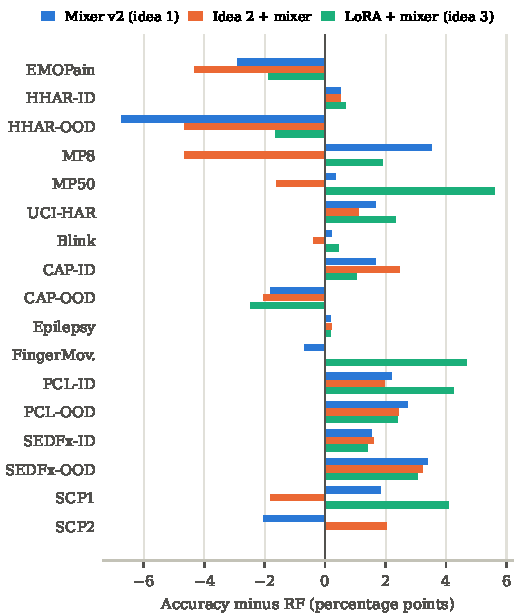
\includegraphics[width=\columnwidth]{figures/gain_over_rf.pdf}
\caption{Accuracy change from the paper's RF protocol for the three improvements (percentage points, mean of 3
seeds). Exact values are in Table~\ref{tab:improve}.}
\label{fig:gain}
\end{figure}


All three improvements keep the pretrained MantisV2 weights frozen. Idea 3 adds a small number of trainable weights
to the encoder. Every trained model uses the same loop:
\begin{itemize}
\item AdamW (learning rate $10^{-3}$, weight decay 0.05), cosine schedule, label smoothing 0.1.
\item Early stopping on a stratified 20\% of the \emph{training} split. The test set is never used for model
selection.
\item 3 seeds per method.
\end{itemize}
Datasets with fewer than 10,000 training samples use up to 100 epochs (patience 20) for heads and 30 for LoRA. Larger
ones use 40 and 4 epochs to fit the free GPU budget.

\textbf{Idea 1: gated cross-channel mixer (Mixer v2).} MantisV2 encodes each channel independently, and the RF sees
only the concatenation. Many of our datasets are multichannel signals in which the relation between channels carries
the label: EEG montages, accelerometer axes, body keypoints. Our head works as follows:
\begin{enumerate}
\item It projects each 512-d channel embedding to 64 dimensions and adds a learned channel embedding.
\item It runs one 2-head self-attention layer across the channels.
\item It adds the result through a residual connection scaled by $\tanh(g)$. The gate $g$ is a learned scalar that
starts at 0.
\item A linear classifier reads the flattened channel vectors.
\end{enumerate}
During training, whole channels are dropped with probability 0.1. The head has 51k--67k parameters depending on $C$
and the number of classes. Our first version used a full transformer layer ($d=128$) with a CLS readout, no gate and no channel dropout. It
overfitted badly:
it lost 4 points on Blink and was unstable across seeds (0.90--1.00). The zero-initialised gate means the model starts
as a plain concatenation head and mixes channels only when the training signal asks for it. The final gate value then
tells us how much mixing each dataset uses.

\textbf{Idea 2: learned layer and token pooling.} The paper fixes layer 2 and a CLS\,+\,mean token after a search on
UCR. We instead keep all 6 layers and 5 tokens per layer (CLS and 4 group means of the patch tokens), 256-d each. A
softmax-weighted sum combines the layers, and attention pooling with 4 learned queries combines the tokens. The
result goes into the Mixer v2 head. The learned layer weights show which depth each dataset prefers.

\textbf{Idea 3: LoRA fine-tuning.} We cut the encoder after layer 2, the layer the paper reads, so layers 3--5 are
never computed. We add rank-8 LoRA adapters \cite{lora} ($\alpha=16$, $B$ initialised to 0) to the QKV and output
projections of layers 0--2. These are 36,864 trainable encoder weights, 0.9\% of the model, and the model starts
exactly at the zero-shot encoder. A Mixer v2 head sits on top. We train with fp16 mixed precision. To fit 50-channel
datasets on a 16\,GB T4, the batch size is capped at $1280/C$ series groups.

% =====================================================================================================
\section{Evaluation of the improvements}\label{sec:results}

\begin{table*}[t]
\caption{Accuracy of the paper's protocol (RF) and our improvements, mean of 3 seeds (logistic regression is
deterministic). All use the same frozen MantisV2 features or encoder. Best per row in bold. ``Head'' is Mixer v2 with
mixing turned off (concatenation + channel dropout). LogReg was not run on CAP.}
\label{tab:improve}
\centering
\footnotesize
\begin{tabular}{rlccccccc}
\toprule
\# & Dataset & RF (paper) & LogReg & Head & Mixer v2 (idea 1) & Pooling (idea 2) & Idea 2 + mixer & LoRA + mixer (idea 3) \\
\midrule
2 & EMOPain & \textbf{.8826} & .8310 & .8469 & .8535 & .8423 & .8394 & .8638 \\
3 & HHAR-ID & .9834 & .9854 & .9859 & .9886 & .9871 & .9885 & \textbf{.9902} \\
4 & HHAR-OOD & \textbf{.5868} & .5604 & .5789 & .5195 & .5319 & .5402 & .5704 \\
5 & MP8 & .6756 & .6521 & .6852 & \textbf{.7109} & .6359 & .6291 & .6947 \\
6 & MP50 & .7092 & .6689 & .7008 & .7126 & .7048 & .6930 & \textbf{.7653} \\
7 & UCI-HAR & .9013 & .9145 & .9102 & .9178 & .9215 & .9125 & \textbf{.9246} \\
8 & Blink & .9956 & .9733 & .9844 & .9978 & .9941 & .9919 & \textbf{1.0000} \\
9 & CAP-ID & .8091 & -- & .8166 & .8258 & .8261 & \textbf{.8336} & .8194 \\
10 & CAP-OOD & \textbf{.7858} & -- & .7488 & .7679 & .7651 & .7653 & .7612 \\
11 & Epilepsy & .9558 & .9311 & .9566 & .9576 & \textbf{.9588} & .9580 & .9575 \\
12 & FingerMovements & .5500 & \textbf{.6400} & .5667 & .5433 & .5533 & .5500 & .5967 \\
13 & PCL-ID & .5769 & .5874 & .5980 & .5988 & .5947 & .5966 & \textbf{.6195} \\
14 & PCL-OOD & .5343 & .5445 & .5478 & \textbf{.5615} & .5465 & .5586 & .5583 \\
15 & SEDFx-ID & .7985 & .8136 & .8042 & .8139 & .8081 & \textbf{.8144} & .8126 \\
16 & SEDFx-OOD & .7640 & .7840 & .7928 & \textbf{.7979} & .7909 & .7962 & .7946 \\
17 & SCP1 & .8134 & \textbf{.8669} & .8305 & .8316 & .7998 & .7952 & .8544 \\
18 & SCP2 & .5148 & .5111 & .5019 & .4944 & .4963 & \textbf{.5352} & .5148 \\
\midrule
 & Mean (17 datasets) & .7551 & -- & .7562 & .7584 & .7504 & .7528 & \textbf{.7705} \\
 & Wins vs.\ RF & -- & 8 / 15 & 11 / 17 & 12 / 17 & 9 / 17 & 9 / 17 & \textbf{13 / 17} \\
 & Best of all methods & 3 & 2 & 0 & 3 & 1 & 3 & \textbf{5} \\
\bottomrule
\end{tabular}
\end{table*}

\begin{figure}[!t]
\centering
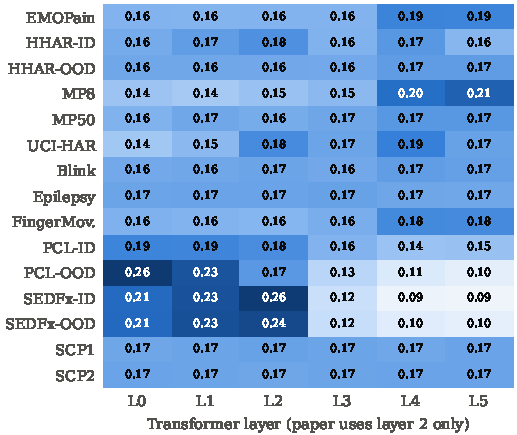
\includegraphics[width=\columnwidth]{figures/layer_weights.pdf}
\caption{Learned softmax weight of each transformer layer in idea 2 (mean of 3 seeds). Uniform is 0.167. Sleep-EDFx
and PCL concentrate on the early layers; MP8 prefers the last ones. (CAP is not shown: it was run with an earlier
script that saved the weights of one seed only.)}
\label{fig:layers}
\end{figure}


\textbf{Overall.} Table~\ref{tab:improve} gives the results on all 17 datasets and Fig.~\ref{fig:gain} the change
from the paper's protocol. LoRA + mixer is the best method overall: mean 0.7705 against 0.7551 for the RF
($+1.5$\pts), better than the RF on 13 of 17 datasets, and best of all seven methods on 5. Its largest gains are MP50
($+5.6$\pts), FingerMovements ($+4.7$), PCL-ID ($+4.3$) and SCP1 ($+4.1$). The mixer on frozen features is cheaper and
improves the mean by $+0.3$\pts. It is the best method on MP8 ($+3.5$), PCL-OOD ($+2.7$) and Sleep-EDFx-OOD ($+3.4$),
and beats the RF on 12 of 17 datasets. Learned pooling alone does not help on average ($-0.5$\pts). Combined with
the mixer it is best on CAP-ID ($+2.5$), Sleep-EDFx-ID and SCP2.

\textbf{Is the cross-channel mixer used?} The gate $\tanh(g)$ answers this directly; its sign is arbitrary, so we use
$|\tanh g|$. With channel mixing on and off in the same head (``Head'' versus ``Mixer v2''), mixing helps on 14 of 17
datasets. The learned gate is largest on HHAR (0.12--0.18), CAP (0.11--0.15), MP8 (0.13--0.14) and Sleep-EDFx (0.15--0.16).
It stays near zero on FingerMovements and SCP1/2 ($\le$0.06), where the training sets have 200--300 samples. The model
therefore learns \emph{when} to use cross-channel structure. The largest single gain from mixing is on MP8 (+2.6
points over the same head without mixing), where the label depends on the relative motion of body keypoints. This
supports our hypothesis that the channel-independent design of MantisV2 leaves accuracy on the table for
multichannel data.

\textbf{Which layers matter?} Fig.~\ref{fig:layers} shows the learned layer weights of idea 2. On most small datasets
they stay almost uniform ($\approx$1/6), so no single layer is clearly better and the fixed layer-2 choice is
reasonable but not special. On the large EEG datasets the head learns a clear preference. On Sleep-EDFx and PCL-OOD,
layers 0--2 receive about two-thirds of the weight (0.66--0.70) and the last layers about 0.1 each. On MP8 and EMOPain the head prefers
layers 4--5 instead. This agrees with the paper's finding that intermediate layers transfer better for EEG. It also
shows that the best depth depends on the domain, which one fixed layer cannot capture.

\textbf{Where the improvements fail.} The RF stays best on EMOPain, HHAR-OOD and CAP-OOD.
\begin{itemize}
\item HHAR-OOD (phones to smartwatch) and CAP-OOD (a new recording machine) are the strongest domain shifts in our set.
Our heads select their checkpoint on held-out \emph{training-domain} data, so they fit the training devices more
closely than the RF does.
\item On the other two OOD tasks, a shift in age (Sleep-EDFx) or in dataset (PCL), every trained head beats the RF.
So the risk depends on the type of shift.
\item On HHAR-OOD, LoRA (4 epochs, the large-data setting) loses only 1.6 points. It also keeps the zero-shot encoder
as its starting point, which suggests that a short fine-tune is safer than a deep head under device shift.
\end{itemize}
On the smallest EEG sets (FingerMovements, SCP1, 268--316 training samples), logistic regression is best: with so few
samples, a simple linear model on good frozen features beats every trained head.

\begin{table*}[t]
\caption{Time per dataset and step (seconds; 3 seeds for each method, LogReg 1 run). Feat./Tok. = one frozen-encoder
pass for the 512-d features (RF, LogReg, Head, Mixer) or for all layers and tokens (Pool, Pool+mix); the methods are
timed with these already computed, except LoRA, which runs the encoder in every epoch. T4 GPU unless marked
$^\dagger$ (CPU-only reproduction notebook); the RF always runs on the CPU cores. -- = not recorded; CAP-ID and
CAP-OOD share one feature pass. Trainable parameters: Head/Mixer 51k--67k, Pool+mix 86k--102k, LoRA +36,864 in the
encoder.}
\label{tab:cost}
\centering
\footnotesize
% generated by kit/make_timing_table.py
\begin{tabular}{lrrrrrrrrrr}
\toprule
Dataset & Feat. & Tok. & RF & LogReg & Head & Mixer & Pool & Pool+mix & LoRA & Total \\
\midrule
EMOPain & 6 & 9 & 21 & 17 & 8 & 11 & 33 & 28 & 404 & 9\,min \\
HHAR-ID & 12 & 17 & 98 & 6 & 47 & 85 & 77 & 139 & 888 & 23\,min \\
HHAR-OOD & 13 & 19 & 119 & 4 & 11 & 15 & 26 & 32 & 155 & 7\,min \\
MP8 & 3 & 4 & 17 & 5 & 12 & 18 & 27 & 30 & 185 & 5\,min \\
MP50 & 16 & 24 & 37 & 4 & 15 & 23 & 121 & 163 & 1,200 & 27\,min \\
UCI-HAR & 111$^\dagger$ & -- & 57$^\dagger$ & -- & 26 & 57 & 191 & 280 & 289 & 17\,min \\
Blink & 16$^\dagger$ & 1 & 2$^\dagger$ & -- & 4 & 7 & 9 & 13 & 41 & 2\,min \\
CAP-ID & 3,386$^\dagger$ & -- & 1,596$^\dagger$ & -- & 16 & 29 & 227 & 234 & 1,163 & 1.8\,h \\
CAP-OOD & -- & -- & 1,681$^\dagger$ & -- & 19 & 30 & 237 & 250 & 1,220 & 57\,min \\
Epilepsy & 48$^\dagger$ & -- & 1$^\dagger$ & -- & 1 & 1 & 5 & 3 & 10 & 1\,min \\
FingerMov. & 45$^\dagger$ & 3 & 6$^\dagger$ & -- & 8 & 3 & 11 & 10 & 136 & 4\,min \\
PCL-ID & 166 & 245 & 688 & 204 & 37 & 38 & 298 & 289 & 1,678 & 1.0\,h \\
PCL-OOD & 149 & 216 & 465 & 155 & 81 & 92 & 599 & 727 & 5,075 & 2.1\,h \\
SEDFx-ID & 138 & 195 & 3,753 & 378 & 136 & 240 & 290 & 325 & 1,472 & 1.9\,h \\
SEDFx-OOD & 123 & 187 & 3,395 & 341 & 125 & 210 & 251 & 282 & 1,371 & 1.7\,h \\
SCP1 & 10 & 1 & 2 & 1 & 9 & 3 & 5 & 6 & 22 & 1\,min \\
SCP2 & $<$1 & 1 & 2 & 2 & 1 & 2 & 1 & 2 & 13 & $<$1\,min \\
\midrule
Sum & 4,242 & & 11,940 & 1,117 & 556 & 864 & 2,408 & 2,813 & 15,322 & \\
\bottomrule
\end{tabular}

\end{table*}

\textbf{Cost.} Table~\ref{tab:cost} gives the time of every step. Summed over the 17 datasets, the paper's RF
took 3.3\,h, LogReg 19\,min, the head 9\,min, the mixer 14\,min, idea 2 (with the mixer) 47\,min and LoRA 4.3\,h.
Feature extraction is cheap on a GPU: 138\,s for the 211,856 Sleep-EDFx-ID samples, against 56\,min on the CPU for
CAP. The mixer head trains in seconds to a few minutes.
On Sleep-EDFx-ID it is 15$\times$ faster than the RF and 1.5 points more accurate, an improvement in both accuracy and
computational cost. LoRA is the most expensive because it runs the encoder (cut to 3 layers) in every epoch, so its
cost grows with channels $\times$ samples. It took 85 minutes for 3 seeds on PCL-OOD, with 48 channels. It is still a
small model to store: the adapters are 147\,KB per task, and the shared encoder is unchanged.

\textbf{Limitations.}
\begin{itemize}
\item We used one training recipe for all datasets, without per-dataset tuning, and only 4 LoRA epochs on large
datasets. The large-data numbers are therefore conservative.
\item Seeds vary the head initialisation and the validation split, not the train and test split.
\item We did not run statistical tests across datasets, and with 17 datasets the mean differences between the mixer
variants (0.2--0.8 points) are not conclusive.
\item Ego4D is missing.
\end{itemize}

% =====================================================================================================
\section{Conclusion}

The MantisV2 zero-shot results reproduce well. Using the public code and data, we match 15 of 17 dataset results
within 0.01, and the remaining gaps trace to data versions and unreported split seeds. Our main lessons are:
\begin{itemize}
\item Report every split seed and every data preprocessing step.
\item Small benchmarks such as FingerMovements cannot separate models.
\item The paper's RF head is neither the most accurate nor the fastest choice on its own features.
\end{itemize}
Keeping the encoder frozen, a gated cross-channel mixer gives most of the gain at almost no cost, and its gate shows
which datasets need cross-channel modelling. Rank-8 LoRA on 0.9\% of the encoder weights gives the best mean
accuracy (+1.5 points over the paper's protocol, 13 of 17 wins). Future work could add domain-robust model selection
for OOD tasks, per-domain layer selection, and cross-channel attention inside the pretrained encoder. All code,
notebooks, and results, with a table comparing our numbers to the paper's, are at \repo.

% =====================================================================================================
\clearpage
\section*{Work plan and contributions}

% TODO (group): check every line below and fill in the bracketed parts before submitting.

\textbf{Work plan.}

\smallskip
\noindent\footnotesize
\begin{tabular}{@{}p{0.27\columnwidth}p{0.68\columnwidth}@{}}
\toprule
When & Work \\
\midrule
Sep 2026 (wk 2--3) & Choose paper (Mantis / MantisV2), check code, checkpoint and GPU access; approval by the lecturer. \\
Oct 2026 & Read MantisV2 and the datasets of Tables 2--3; plan the split of datasets: Aadil 1--6, Padmanabh 7--12,
Praneet 13--18. \\
6 Nov & Reproduction of datasets 7--12 (Colab, then Kaggle CPU). \\
6 Nov & Improvement run 1 (first mixer and pooling; overfitted), Mixer v2, then idea 2 on CAP and LoRA on datasets
7--12 (Kaggle GPU). \\
6--7 Nov & Reusable kit (\texttt{src/mantisv2\_kit.py}); runs on datasets 1--6 and 13--18 in 5 parallel Kaggle notebooks; memory fixes
and re-runs; final tables. \\
7--16 Nov & Report writing, figures, review; README check; submission on Brightspace by 16 Nov. \\
\bottomrule
\end{tabular}
\normalsize

\medskip
\textbf{Work division and final contributions.}
\begin{itemize}
\item \textbf{Padmanabh Khunt:} reproduction of datasets 7--12; design and code of the three improvements; the
kit and the Kaggle runs for datasets 1--6 and 13--18; GitHub repository and README; [report sections].
\item \textbf{Aadil [surname]:} [planned: datasets 1--6; actual contribution to be filled in by the group].
\item \textbf{Praneet [surname]:} [planned: datasets 13--18; actual contribution to be filled in by the group].
\end{itemize}
% TODO (group): if the module asks you to declare the use of AI tools, add the statement here.

% =====================================================================================================
\clearpage
\begin{thebibliography}{99}
\footnotesize

\bibitem{mantisv2} V.~Feofanov, S.~Wen, J.~Zhang, L.~Pan, and I.~Redko, ``MantisV2: Closing the zero-shot gap in
time series classification with synthetic data and test-time strategies,'' arXiv:2602.17868, 2026.

\bibitem{mantis} V.~Feofanov \emph{et al.}, ``Mantis: Lightweight calibrated foundation model for user-friendly time
series classification,'' arXiv:2502.15637, 2025.

\bibitem{lora} E.~J.~Hu \emph{et al.}, ``LoRA: Low-rank adaptation of large language models,'' in \emph{Proc. ICLR},
2022.

\bibitem{woods} J.-C.~Gagnon-Audet, K.~Ahuja, M.~J.~Darvishi~Bayazi, P.~Mousavi, G.~Dumas, and I.~Rish, ``WOODS:
Benchmarks for out-of-distribution generalization in time series,'' \emph{Trans. Mach. Learn. Res.}, 2023.

\bibitem{tfc} X.~Zhang, Z.~Zhao, T.~Tsiligkaridis, and M.~Zitnik, ``Self-supervised contrastive pre-training for time
series via time-frequency consistency,'' in \emph{Proc. NeurIPS}, 2022.

\bibitem{uea} A.~Bagnall \emph{et al.}, ``The UEA multivariate time series classification archive, 2018,''
arXiv:1811.00075, 2018.

\bibitem{fm4mtsc} S.~Isiacik \emph{et al.}, ``An empirical evaluation of foundation models for multivariate time
series classification,'' 2025. Code and data: \url{https://github.com/mlgig/FM4MTSC}.

\bibitem{bakeoff} M.~Middlehurst, P.~Sch\"afer, and A.~Bagnall, ``Bake off redux: A review and experimental
evaluation of recent time series classification algorithms,'' \emph{Data Min. Knowl. Discov.}, vol.~38, 2024.

\bibitem{moment} M.~Goswami, K.~Szafer, A.~Choudhry, Y.~Cai, S.~Li, and A.~Dubrawski, ``MOMENT: A family of open
time-series foundation models,'' in \emph{Proc. ICML}, 2024.

\bibitem{minirocket} A.~Dempster, D.~F.~Schmidt, and G.~I.~Webb, ``MiniRocket: A very fast (almost) deterministic
transform for time series classification,'' in \emph{Proc. KDD}, 2021.

\bibitem{rf} L.~Breiman, ``Random forests,'' \emph{Mach. Learn.}, vol.~45, pp.~5--32, 2001.

\bibitem{pineau} J.~Pineau \emph{et al.}, ``Improving reproducibility in machine learning research,'' \emph{J. Mach.
Learn. Res.}, vol.~22, no.~164, pp.~1--20, 2021.

\bibitem{ego4d} K.~Grauman \emph{et al.}, ``Ego4D: Around the world in 3,000 hours of egocentric video,'' in
\emph{Proc. CVPR}, 2022.

\end{thebibliography}

\end{document}
